% FEUP THESIS STYLE for LaTeX2e
% how to use feupteses (changed from the original for MIEEC)
%
% FEUP, JCL & JCF, Tue May 20 18:53:15 2008
%
% PLEASE send improvements to jlopes at fe.up.pt, jcf at fe.up.pt

%%========================================
%% Commands: pdflatex thesis
%%           bibtex thesis
%%           makeindex thesis (only if creating an index) 
%%           pdflatex thesis
%%========================================
\documentclass[11pt,a4paper,twoside,openright]{report}
\usepackage[utf8]{inputenx}
\usepackage[official]{eurosym}
\usepackage[english]{babel}
\usepackage{amsmath}
\usepackage{amsfonts}
\usepackage{tkz-graph}
\usepackage{multirow}
\usetikzlibrary{calc,arrows,shapes}

\usepackage{enumerate}

%% For the final version, comment next line and uncomment the second line
%\usepackage[provisional,numericrefs]{feupteses}
\usepackage[alpharefs]{feupteses} 

%% Options: 
%% - portuges: titles, etc in portuguese
%% - provisional: the thesis has not been approved yet
%% - alpharefs: bibliography references are alphabetic
%% - numericrefs: bibliography references are numbered (in order of citation)
%% ( by default: author-date format of the ``natbib'' package is used 
%%   the portuguese version requires the file ``plainnat-pt.bst'' to be 
%%   present in the same directory )

%% Include MIEIC definitions different from standard style
\usepackage{mieicpatch}

\version{1.0}

%% Uncomment in the final version in order to make version footer disappear
%% \noversiontrue
%% Uncomment to create an index (at the end of the document)
\usepackage{makeidx}
\makeindex
%% Path to the figures directory
%% TIP: use folder ``figures'' to keep all your figures
\graphicspath{{figures/}}

%%========================================
%% Macros
% format
\newcommand{\class}[1]{{\normalfont\slshape #1\/}}

% entities
\newcommand{\Feup}{Faculdade de Engenharia da Universidade do Porto}
\newcommand{\ProjectAuthor}{Gonçalo Santarém da Silva}
\newcommand{\ProjectSupervisor}{Ademar Manuel Teixeira de Aguiar}

% names
\newcommand{\ProjectName}{Scaling Rails: a system-wide approach to performance optimization}
\newcommand{\headermark}[1]{\chaptermark{\uppercase{#1}}}

% Gantt
\newcommand\ganttline[4]{% line, tag, start end
\node at (0,#1) [anchor=base east] {#2};
\fill[gray] (#3/15,#1-.2) rectangle (#4/15,#1+.2);
\draw[black,thick] (#3/15,#1-.2) rectangle (#4/15,#1+.2);}

%%========================================

%%========================================
%% Start of document
%%========================================
\begin{document}
  %%----------------------------------------
  %% Information about the work
  %%----------------------------------------
  \title{\ProjectName}
  \author{\ProjectAuthor}
  \degree{State of the Art Review\\[2mm]
  Master in Informatics and Computing Engineering}
  %% Date of submission
  \thesisdate{29$^{th}$ January, 2010}

  %% Insert copyright text if used
  %\copyrightnotice{Name of the Author, 2008}

  \supervisor{Supervisor}{\ProjectSupervisor}{(PhD.)}
  %% Uncomment next line if necessary
  %% \supervisor{Second Supervisor}{Filipe Abrantes}{(PhD.)}

  %% Uncomment committee stuff in the final version
  %\committeetext{Approved in oral examination by the committee:}
  %\committeemember{\textbf{Chair}}{Ana Paula Cunha da Rocha}{(Auxiliar Professor)}
  \signature
  %\committeemember{\textbf{External Examiner}}{Carlos Miguel Ferraz Baquero Moreno}{(Auxiliar Professor)}
  %\committeemember{\textbf{Internal Examiner}}{Ademar Manuel Teixeira de Aguiar}{(Auxiliar Professor)}
  %\committeedate{17$^{th}$ July, 2009}

  %% Specify cover logo (in folder ``figures'')
  \logo{feup-logo.pdf}

  %%----------------------------------------
  %% Cover page(s)
  %%----------------------------------------
  \maketitle
  %% Uncomment next line in the final version
  \committeepage

  %% Preliminary materials
  \StartPrelim
  \begin{singlespace}
    % TODO: Review at the end

\chapter*{Abstract}
\pdfbookmark[0]{Abstract}{abstract}

Web's popularity and importance on everyday life increases day by day. Its users create new standards and expectations, demanding better user experiences in their daily interactions. Availability and response times are key factors to every website's success. The noticeable Web growth encouraged the creation of better tools to improve the quality of web applications. One of this tools is Ruby on Rails, a framework built on top of the Ruby programming language.

Rails scalability is questionable since many platforms experienced performance and availability difficulties when having to respond to increased popularity. One of these platforms was Twitter. 

Rails performance is dependent on all the underlying components like the operating system, ruby, web server, database, rails itself and its superjacent application. A key concept in Rails' performance tuning and optimization is to analyze and improve each component from the framework's point of view. No component should be optimized as an individual, independent part --- the whole system must be taken into account when optimizing, considering each component's sensitive dependencies.

This report is a review on the state of the art in scaling Rails. It starts by exposing reliable software alternatives to each component and explains their characteristics, principles, philosophies and architecture, providing a solid base for their analysis. Their state of the art is reviewed, exhibiting related work and its results. A problem-solving approach to this issue is then proposed, along with its respective scheduling which will be endured at \textit{Escolinhas}, an expanding Ruby on Rails application. Finally, an analysis is performed on the aforementioned related work and future options are narrowed down according to other research's results.

\chapter*{Resumo}
\pdfbookmark[0]{Resumo}{resumo}

A popularidade e importância da Web na vida quotidiana aumenta de dia para dia. Os seus utilizadores criam novos padrões e expectativas, exigindo melhores experiências de utilização na sua interacção com a plataforma. A disponibilidade e tempo de resposta de um sítio na Internet revelam-se como sendo factores críticos de sucesso. O notório crescimento da Web motivou a criação de melhores ferramentas que permitissem desenvolver aplicações com qualidade superior. Uma destas ferramentas é o Ruby on Rails, escrita na linguagem de programação Ruby.

A escalabilidade do Rails é questionável já que várias plataformas apresentaram problemas de eficiência e disponibilidade quando viram a sua popularidade aumentada. Uma destas plataformas foi o Twitter.

O desempenho do Rails depende de todos os seus componentes subjacentes como o sistema operativo, o ruby, o servidor web, a base de dados, o próprio Rails e a aplicação sobrejacente. Um conceito fundamental na optimização de desempenho do Rails consiste em analisar e melhorar cada componente do ponto de vista do Rails. Nenhum componente deve ser optimizado como se fosse uma parte independente do sistema --- todos os componentes devem ser tidos em conta quando se optimiza, tendo sempre em conta o impacto que estes poderão ter nos restantes.

Neste relatório é apresentada uma revisão do estado da arte sobre a escalabilidade do Rails. Começa-se por expor alternativas viáveis para cada componente e explica-se as suas características, pormenores e arquitectura, criando uma base sólida para a sua análise. O estado da arte de cada uma destas alternativas é então revisto, expondo trabalhos relacionados e as suas conclusões. Uma aproximação à solução deste problema é proposta, acompanhada da sua calendarização, que será aplicada no contexto do \textit{Escolinhas}, uma aplicação em crescimento desenvolvida em Ruby on Rails. Por fim, é feita uma análise sobre as alternativas supracitadas e estas são limitadas pelas descobertas feitas em projectos realizados.

    %\chapter*{Acknowledgements}
\section*{}
To everyone at \textit{Escolinhas.pt}, for allowing me to mix work and fun on a daily basis.\\
\mbox{}\\
To Ademar Aguiar and Nuno Baldaia, for their patience at guiding a sometimes slugabed student.\\
\mbox{}\\
To Muhammed Ali, for helping me set my priorities when coding tons of C was what I really wanted to do.\\
\mbox{}\\
To Brian Lopez, for happily sharing his knowledge on Ruby C extensions when all the documentation I could find was written in Japanese.\\
\mbox{}\\
To Rupak Ganguly, for helping me polish and publish my first magazine article ever.\\
\mbox{}\\
To Yehuda Katz, for guiding me through the Ruby Summer of Code and trusting me every single time, even when it meant breaking Rails.\\
\mbox{}\\
To Pedro Coelho, for lending me his computer when all official means have failed.\\
\mbox{}\\
To Paulo Pereira, for revising this report, pointing me in the right direction when I started and for continuously motivating me.\\
\mbox{}\\
To everyone who stained their black cloaks with me, for teaching me things I could not have learned elsewhere.\\
\mbox{}\\
To Sara, for all her love, help and support, for cheering me up whenever I felt down and for making me feel like I am the best person in the world.\\
\mbox{}\\
To my family, for their patience and support while I pulled dozens of all nighters during this awesome course, and for giving me the possibility to make the most out of it.\\

    \cleardoublepage
\thispagestyle{plain}

\vspace*{8cm}

\begin{flushright}
  \emph{``Fast isn`t a feature. Fast is a requirement.''} \\
  \vspace*{1.5cm}
  --- Jesse Robbins
\end{flushright}

%% Success is not about scale, it’s about sustainable execution
%% Jeff Putz
    % initial quotation if desired
    \cleardoublepage
    \pdfbookmark[0]{Table of Contents}{contents}
    \tableofcontents
    \cleardoublepage
    \pdfbookmark[0]{List of Figures}{figures}
    \listoffigures
    \cleardoublepage
    \pdfbookmark[0]{List of Tables}{tables}
    \listoftables
    \cleardoublepage
    \pdfbookmark[0]{Definitions}{def_defs}
    \chapter*{Definitions} % (fold)
\label{cha:definitions}
\headermark{Definitions}
The following definitions are in order of appearance.\\\\

\begin{description}
  \item[World Wide Web] System of interlinked hypertext documents contained on the Internet.
  \item[Coupling] The degree to which each program module relies on each one of the other modules.
  \item[Continuations] C-like gotos for Ruby.
  \item[Fork] A processes' act of creating a copy of itself.
  \item[Endian] Order of individually addressable sub-units within a longer data word in external memory.
  \item[Green threads] Threads scheduled by the Virtual Machine, emulating multi-threaded environments.
  \item[Mark and Sweep] The first garbage collection algorithm, consisting of two blocking phases --- a mark phase and a sweep phase.
  \item[Just-in-time compilation] Also known as dynamic translation, just-in-time compilation is the act of converting code at runtime prior to executing it natively.
  \item[Ahead-of-time compilation] Compilation of intermediate code into a system-dependent binary.
  \item[EventMachine] A library for Ruby, C++ and Java that provides event-driven I/O using the Reactor pattern.
\end{description}

% chapter definitions (end)

    \cleardoublepage
    \pdfbookmark[0]{Abbreviations}{def_abbr}
    \chapter*{Abbreviations} % (fold)
\label{cha:abbreviations}
\headermark{Abreviations}
The following abbreviations are in alphabetical order.\\\\

\begin{description}
  \item[AJAX] Asynchronous JavaScript and XML
  \item[API] Application Programming Interface
  \item[CERN] \textit{Conseil Européen pour la Recherche Nucléaire}, currently known as European Organization for Nuclear Research
  \item[CFQ] Completely Fair Queuing
  \item[CPU] Central Processing Unit
  \item[CSV] Comma-Separated Values
  \item[DBMS] Database Management System
  \item[DRY] Don't Repeat Yourself
  \item[ERB] Embedded Ruby
  \item[HTTP] Hypertext Transport Protocol
  \item[IP] Internet Protocol
  \item[I/O] Input/Output
  \item[JVM] Java VM
  \item[MB] Megabyte
  \item[MRI] Matz's Ruby Interpreter
  \item[MVC] Model-View-Controller
  \item[MPM] Multi-Processing Module
  \item[ORM] Object-Relational Mapping
  \item[OS] Operating System
  \item[PID] Process ID
  \item[PHP] PHP Hypertext Preprocessor
  \item[POSIX] \textbf{P}ortable \textbf{O}perating \textbf{S}ystem \textbf{I}nterface [for Uni\textbf{x}]
  \item[Rails] Ruby on Rails
  \item[RDBMS] Relational DBMS
  \item[REE] Ruby Enterprise Edition
  \item[STL] Standard Template Library
  \item[TCP] Transmission Control Protocol
  \item[UNIX] Uniplexed Information and Computing Service
  \item[USA] United States of America
  \item[VCS] Version Control Systems
  \item[VM] Virtual Machine
  \item[Web] World Wide Web
  \item[YARV] Yet Another Ruby VM
  \item[.NET] Microsoft .NET Framework
\end{description}

% chapter abreviations (end)



  \end{singlespace}

  %%----------------------------------------
  %% Body
  %%----------------------------------------
  \StartBody

  %% Introduction
  \chapter{Introduction} % (fold)
\label{cha:introduction}
\headermark{Introduction}

\section*{} % (fold)
This section briefly presents the project's context, purpose and scope. It covers the motivation behind it and its objectives.% while also detailing the report structure, providing an overview of each of the remaining chapters.

% section  (end)

\section{Context} % (fold)
\label{sec:context}
The internet started in the early 1990s as a work tool for CERN. It evolved into a vast information repository for the public~\cite{teaching_webdev_web20}---the Web---and had 16 million users back in 1995. Next year Netscape went public and achieved an impressive 90\% market share. It quickly lost it's prominence during the first browser war, conceding its leadership to Microsoft's Internet Explorer~\cite{browser_wars}. The Web was starting to become a presence in everyday life. In 2009, 14 years later, the Web had more than 1700 million users and its popularity keeps growing nowadays~\cite{internet_stats}.

The Web is becoming an essential pillar of many businesses, social networks, gaming industries \textit{et al.} since distance is no longer an issue when it comes to information exchange.  It begins to present itself as a critical presence on computers nowadays. Many people believe future applications will mostly be web-based, pushing the internet importance even further~\cite{browser_application_platform}.

The growth of internet usage and its impact in corporate applications implies all kinds of particularities. First of all, users must trust the web. This is an essential pillar of any web service. To build costumer trust, providing services must pay attention to their users needs and desires and they must meet their user's expectations~\cite{trust_semantic_web}. 

In the fall of 2001, many people concluded that the web was overhyped and bloated. There was the need for richer content and better user experiences~\cite{oreilly_web20}. In this context, the term \textit{Web 2.0} was born. Its meaning is not well defined but a common definition consists in the improvement of the first version of the Web~\cite{rubyonrails_tutorial} and involves many core concepts like usability and dynamic content~\cite{what_is_web20}.

Side by side with the Web growth was the increasing user's expectations when it comes to user experience. As time goes by, users demand better interaction with the services they use as part of their user experience is based on response times~\cite{prioritizing_web_usability}, responsiveness and performance of Web applications. These concepts become part of the key factors to their success~\cite{responsiveness}. Users expect waiting times to kept at an acceptable minimum and whenever they feel that this expectation isn't being met their trust on the service diminishes. When users enter a given website they have a limited patience, related to their expectations and previous experiences. Whenever the system fails to meet those expectations, their patience gets smaller and it can cause them to leave. Steve Krug calls this the \textit{Reservoir of Goodwill}~\cite{dont_make_me_think}.

This increasing popularity, dependence and demand on the Web strives the developers for better tools to build quality web applications. Most developers seek the ability to increase their productivity while being able to build more complex, full-featured systems that suit their user's need, either it's a social or business-oriented service~\cite{comparison_agile_frameworks}.

With the growing importance of Web applications, many tools emerged trying to make the developer's life easier. \textit{Web 2.0} improved the internet and created a new set of needs and expectations. This need motivated the development of powerful frameworks and, among many others, the Ruby on Rails framework was born~\cite{what_is_web20}. As ~\cite{rubyonrails} puts it:
\begin{quote}
  ``Ruby on Rails$^{\scriptsize \textregistered}$~is an open-source web framework that's optimized for programmer happiness and sustainable productivity. It lets you write beautiful code by favoring convention over configuration.''
\end{quote}
Ruby on Rails is one of the best-known Ruby frameworks~\cite{agile_webdevelopment_with_rails}. Most people and companies want a \textit{Web 2.0} killer application and Rails seems an excellent way of doing it~\cite{oo_business_models}. This framework is commonly associated with the \textit{Web 2.0} concept, along with AJAX~\cite{spaghetti_code}. It is also deeply related with \textit{Agile Web Development}~\cite{agile_webdevelopment_with_rails}. Rails allows developers to build high quality applications with smaller effort – less time, less lines of code and less files, always with low coupling~\cite{maintainability_web_applications_j2ee_dotnet_ror}.

As~\cite{oreilly_ror} states:
\begin{quote}
  ``Ruby on Rails is a breakthrough in lowering the barriers of entry to programming. Powerful web applications that formerly might have taken weeks or months to develop can be produced in a matter of days.''
\end{quote}
The huge framework's success had it jumped into a spotlight with many companies starting to use it as the development framework for their applications. Some widely known services like \textit{Basecamp}, \textit{Twitter}, \textit{Hulu}, \textit{YellowPages} or \textit{Github} push this platform even further by giving it even more popularity~\cite{rubyonrails_applications}.

\begin{description}
  \item[Basecamp,] the original Rails application~\cite{rubyonrails_applications}, is an online project management tool which features live collaboration and task aiding software~\cite{basecamp}. It has over 1 million users since 2006~\cite{basecamp_turns_1000000}. It is ranked 680$^{th}$ on the Alexa Traffic Rank~\cite{alexa}.
  \item[Twitter,] a real-time short messaging service that works on multiple networks and devices. It's used for quick sharing of information, either updates from friends or breaking world news updates~\cite{twitter}. It had more than 18 million adult users in the USA by the end of 2009 and is expected to achieve an impressive quantity of 26 million adult users in the same country by 2010~\cite{emarketer_twitter_usage}. It is ranked 12$^{th}$ on the Alexa Traffic Rank~\cite{alexa}.
  \item[Hulu,] a TV and Movie streaming website which allows users to watch their favorite videos on the browser for free~\cite{hulu}. It had a significant amount of traffic in 2009, only staying behind Google services and Fox Interactive Media~\cite{hulu_growth}. It ranks 160$^{th}$ on the Alexa Traffic Rank~\cite{alexa}.
  \item[YellowPages,] a service that indexes and provides business listings of the United States of America, allowing users to search for services they're looking for, among other features.~\cite{yellowpages}.  It ranks 757$^{th}$ on the Alexa Traffic Rank. To note that it is a USA-oriented application, raking 161$^{th}$ if the scope is limited to the USA~\cite{alexa}.
  \item[GitHub,] one of the best know repository hosting system which works with the Git VCS. It currently has more than 185 thousands of registered developers and it is associated with public, open source projects but also proprietary codes ~\cite{github}. It ranks 1390$^{th}$ on the Alexa Traffic Rank~\cite{alexa}.
\end{description}
These systems have high scalability demands. In order to keep increasing their popularity and to keep building users trusts, they also need to provide a great user experience along with reasonable response times while serving thousands of requests concurrently.

Some press reports question Rails' ability to scale, mainly based on the issues \textit{Twitter} faced when its growth reached a given magnitude~\cite{interview_alex_payne}. However, most of the issues were demystified as a software architecture design issue, taking the blame off of Ruby on Rails~\cite{ror_ecosystem_whitepaper}. Nonetheless, despite all the advantages this framework possesses, scalability isn't one of them. Ruby isn't as scalable as PHP or Java but on the other hand offers the higher development speed~\cite{issues_web_frameworks}. Luckily, only high traffic websites like \textit{Twitter} have to get deeply involved with scalability but it's still an issue to be addressed.

Developers should be able to build Rails-based high-quality applications whose scaling isn't directly related to hardware upgrades~\cite{interview_alex_payne}. Issues should be identified and solved so that this acclaimed Ruby framework becomes more scalable \textit{out of the box}, diminishing its dependence on hardware upgrades or major architectural refactoring. This way, Ruby on Rails development happiness can last through the whole process of creation and maintenance of a web platform.
% section context (end)


\section{Motivation and Objectives} % (fold)
\label{sec:motivation_and_objectives}
The Web starts to play a really important role in many people's lives, either from a professional or personal point of view. User experience has become of great importance in recent times, with the \textit{Web 2.0} raising the expectations on a better interaction.

Internet accesses keep growing and the recent developments in the smart phone, tablet and notebook's areas help increasing this number even further, with people starting to be permanently connected to the internet~\cite{npd:3g,mobileweb,netbooks}.

Users expect the Web to work as they pre-conceived and this important detail has a great focus on recent developments in Interaction Design~\cite{interaction_design}. As innovation keeps pushing user experiences to a new level, with richer information presented and organized in ways never seen before, technologies tend to emerge to support such evolutionary content and organization. Developers need to meet the users' needs and they don't have unlimited time to do it, thus many recent frameworks have gained notorious popularity for being agile and robust, bringing productivity indices to a higher level~\cite{trends_webdev}. Ruby on Rails, as most recent frameworks, offers convenient methods and features which greatly improve the product's quality without the need for extended development times. However, it also makes it harder for the development team to fully optimize the application when there are limited hardware resources~\cite{look_common_performance_problems_rails}.

Scaling and performance optimization shouldn't be so hard to achieve in Rails, though. As many \textit{Web 2.0} platforms are born, a few built using Ruby on Rails, some might succeed and Rails shouldn't be an obstacle to their success. Rails' purpose is to help developing high-quality applications, not limiting their accomplishments to a given number of concurrent users or high response times. The Web should be able to shine in all of its glory and tools like Ruby on Rails are here to allow it to improve and innovate further and further, meeting the users' increasing standards and demands.

Performance optimization has been a work focus since computers were born~\cite{mass_memory_system_optimization}. Many have optimized all the gears involved in making Rails work, like the Ruby interpreter~\cite{yarv}, Rails itself~\cite{rails_merb_merge_performance} or the superjacent application~\cite{scaling_rails_bottomup,vaporware_to_awesome,rebuilding_scaling_yellowpages,5tips_scale_ror}. Many have focused on improving speed and scalability of databases~\cite{performance_analysis_db_arch} and webservers~\cite{webserver_scheduling}. Others look for potential issues in the Operating System~\cite{unix_os_comparison, architecture_impact_os} and end up patching and tweaking the system's configuration. One can infer that most of the performance optimization activities focus on single elements or try to find out a single culprit to blame. It is also necessary to envision performance optimization as a globalist activity. If an intervenient changes it will affect all those who interact with it by smaller or larger margins. In Chaos Theory this is called \textit{Sensitive Dependence} or, as more commonly known, the \textit{Butterfly Effect}. As ~\cite{butterfly_effect_quote} mentions:
\begin{quote}
  ``The exponential divergence (\ldots) from slightly different initial conditions---the famous butterfly effect---is a fingerprint of chaos in classical mechanics.''
\end{quote}
These possible side effects must be taken into account when optimizing the performance of a highly dependent system like Rails. The system should be optimized as a whole, not as a procedure with many, independent steps and components. The whole system performance is what truly matters, not the performance of its individual parts. This is the core mindset of this project.

There is need for a solid set of Rails development conventions and guidelines with scaling and performance in mind. Developers also seek optimal configurations for all the components involved so they can wring every processing cycle out of their applications, in order to increase application scalability and decrease response processing times. There is also urgency in looking at all the tools Rails depends on and optimizing them to suit Rails needs---the system, envisioned as a whole.

This philosophy will be applied in \textit{Escolinhas}~\cite{escolinhas}, a growing Portuguese Rails based project. \textit{Escolinhas} aims at sustaining social and collaborative work for children in elementary schools involving students, teachers and parents as its users. With the user demand increasing day by day, it becomes an excellent case-study application to research, test and apply all the work and discoveries made during the course of this thesis.

Concluding, the aim of ``Scaling Rails: a system-wide approach to performance optimization'' is to produce the aforementioned generic conventions and guidelines, to find generalist optimal configurations for the most important components that Rails depends on and to optimize them for the framework at use, all in the Escolinhas~\cite{escolinhas} context mentioned before.
% section motivation_and_objectives (end)


\section{Report Overview} % (fold)
\label{sec:report_overview}
The rest of this report is structured as follows.
\begin{description}
  \item[Chapter~\ref{cha:technologies}: ``Technologies''] gives an overview over this research's possibly involved technologies, providing important background information on each one of them.
  \item[Chapter~\ref{cha:state_of_the_art}: ``State of the Art''] reviews each component's performance and scalability when compared to its alternatives along with a few other details.
  \item[Chapter~\ref{cha:approach}: ``Approach''] suggests a possible approach into tackling the presented issue.
  \item[Chapter~\ref{cha:conclusions}: ``Conclusions''] narrows alternatives down by using related work's conclusions, exposed in the state of the art, to discard certain options.
\end{description}
% section report_overview (end)

% chapter introduction (end)

  %% Technologies
  \chapter{Technologies} % (fold)
\label{cha:technologies}
\headermark{Technologies}

\section*{} % (fold)
This chapter will expose relevant technologies to this research. A high-level analysis will be made concerning their most important characteristics and a solid knowledge base will be provided as a sustaining base for exposing their state of the art.
% section  (end)

\section{Operating Systems}
\label{tech:sec:operating_systems}
The operating system is the base of everything else. It runs on top of the hardware and allows applications to use its resources. There are many kinds of operating systems, with different characteristics and philosophies. The relevant ones to this research will be explained in the following sections.

\subsection{GNU/Linux}
Linux is the term used to describe UNIX-based operating systems that run the Linux \textit{Kernel}. It was created in 1991 by Linus Torvalds~\cite{linux_kernel_evolution}, who is also the author of \textit{git}~\cite{pro_git}. It is one of the most significant open-source projects where volunteers from all over the world work together to achieve a common goal---improve the operating system itself~\cite{linux_kernel_evolution}. While having low usage on desktop systems~\cite{w3counter}, Linux is widely used on servers, mainframes and super computers. Linux is commonly known for its security and reliability. One sustaining example is the list of the most reliable hosting company sites in December 2009, where Linux figures 6 times in the top 10~\cite{netcraft_dec2009}.

Linux stands as the base for many UNIX-like software distributions, specifically Linux distributions. These consist on a large collection of software applications which range from full-featured desktop configurations to minimal environments. Non-commercial Linux distributions commonly used in server environments include:
\begin {description}
\item[Debian,] maintained by a developer community with a strong commitment to free software principles\footnote{\url{http://www.debian.org/}}.
\item[Ubuntu Server,] derived from Debian and maintained by Canonical, being the server version of the most popular Linux distribution\footnote{\url{http://www.ubuntu.com/products/whatIsubuntu/serveredition}}.
\item[CentOS,] derived from the same sources used by \textit{Red Hat}\footnote{\url{http://www.centos.org/}}.
\item[Gentoo,] known for its FreeBSD Ports-like system for application custom compiling\footnote{\url{http://www.gentoo.org/}}.
\end{description}
Each distribution aims at adding its own flavor to the Linux operating system, providing different user experiences to their users~\cite{tuning_costumizing_linux}.


\subsection{Berkeley Software Distribution}
Berkeley Software Distribution, also know as BSD or \textit{Berkeley} \textit{Unix}, is considered to be a branch of the \textit{Unix} operating system. It was created in 1977 in the University of California in Berkley by the Computer Systems Research Group.  Entitled by some as the greatest software ever written~\cite{ greatest_software_ever_written}, even Linux's creator, Linus Torvalds himself, went as far as stating~\cite{ interview_linus}: 
\begin{quote}
  `` If 386BSD had been available when I started on Linux, Linux would probably never had happened''
\end{quote}
Just like Linux, it is open-source software and has several associated distributions, although at a smaller scale. FreeBSD\footnote{\url{http://www.freebsd.org/}} and OpenBSD\footnote{\url{http://www.openbsd.org/}} are among the most popular BSD distributions.

A significant remark is that both Apple's \textit{Mac OS X}~\cite{leopard_os_foundations} and Microsoft's \textit{Windows}~\cite{bsd_code_windows} use parts of BSD's source code.

\subsection{Microsoft Windows Server}
Windows Server is Microsoft Corporation's operating system oriented towards servers. The current version of this operating system is called \textit{Windows Server 2008} and, as its name implies, was released in 2008. It is built on top of the same code base used in \textit{Windows Vista}.

Windows is proprietary software and consequently does not come in a distribution manner like the \textit{UNIX}-based operating systems mentioned before.

\section{Ruby} % (fold)
\label{tech:sec:ruby}
Ruby is a dynamic and object-oriented language created by Yukihiro Matsumoto, who released it to the public in 1995. The purpose was to create a ``language that was more powerful than Perl, and more object-oriented than Python''~\cite{interview_creator_ruby}.

Ruby was inspired by languages such as Lisp, Smalltalk and Perl, and its core characteristics and features are~\cite{ruby_about, ruby_book}:
\begin{description}
  \item[Open source.] Ruby's license allows anyone to use, copy, modify or distribute it.
  \item[Pure object-oriented.] In Ruby, everything is an object, including classes, modules and data types---even numbers, booleans and null values which in other object-oriented languages are known as ``primitives''. An object's properties are known as ``instance variables'' and actions are ``methods''.
  \item[Flexible.] It not only features dynamic typing, but also very powerful reflective and metaprogramming capabilities. Ruby does not restrict what a programmer can do. Any part of Ruby code can be removed, redefined or extended, even at runtime. This is not only true for a programmer's own code, but also for core Ruby classes such as Object and String.
  \item[Automatic memory management.] Like other languages such as Java and contrary to C, developers do not manage the program's memory usage.
  \item[Portable.] Ruby is mainly developed in GNU/Linux but can run on most operating systems and platforms such as BSD, Mac OS X, Windows 95 and many others.
  \item[Exception handling.] Ruby can recover from errors just like Java, C++ or Python.
\end{description}
Ruby started to become popular in 2001, with the start of the~\textit{RubyGems}\footnote{\url{http://rubygems.org/}} project, which allows easy packaging and distribution of applications and libraries~\cite{railssolutions}. Ruby has two main versions and the last one was publicly released approximately two years ago~\cite{ruby191_release}.


\subsection{Ruby 1.8}
The most commonly found version of Ruby in Rails' projects is the 1.8, mainly due to the fact that it was the officially recommended version for many years.

\subsubsection{MRI}
Ruby's 1.8 official interpreter was developed by the language's creator Yukihiro Matsumoto, also known as \emph{Matz} and its first public release happened in 1995. Some people mistake MRI for ``Main Ruby Implementation'' but the abbreviation is actually related to its creator's name---\emph{Matz Ruby Interpreter}. Some particular characteristics of this interpreter include:
\begin{description}
\item[Language.] MRI is written in C.
\item[Threading.] It can emulate a threaded environment without relying on the operating system capabilities by using \textit{green threads}.
\item[Garbage Collector.] The garbage collector is based on the simple \textit{mark-and-sweep} algorithm.
\item[Extensions.]  Developers can extend Ruby's basic functionality by writing their own extensions. These can be written in Ruby or in native C, by using MRI's powerful API.
\item[Bytecode Interpretation.] MRI lacks a bytecode interpreter. When a program is executed, MRI will parse its source and create its syntax tree. Then, it will iterate over this tree directly while executing the program.
\end{description}
It the only official Ruby interpreter for many years and, consequently, it is the most commonly used.


\subsubsection{Ruby Enterprise Edition}
This Ruby interpreter, also called REE, is based on the MRI source code. However, it includes many Rails-oriented enhancements. It was first released in 2003 and has been merging with MRI periodically, keeping its own changes aside. Its characteristics and differences from the official interpreter for version 1.8---MRI---include~\cite{rubyenterpriseedition}:
\begin{description}
\item[Language.] Since REE is based on the MRI, it is written in C.
\item[Threading.] The thread implementation is the same found on MRI.
\item[Garbage Collector.]  The garbage collector was improved, being \textit{copy-on-write} friendly. This allows for reduced memory usage when paired with Passenger, who uses \textit{preforks} in combination with this feature.  It also enables the user to tweak its settings for adaptive performance.
\item[Extensions.]  Just like MRI, it supports Ruby and native C extensions. 
\item[Bytecode Interpretation.] REE is mostly based in MRI's source code, as mentioned before, so it lacks a bytecode interpreter. It also iterates over the program's syntax tree directly.
\item[Other Differences.] REE uses \textit{tcmalloc} for memory allocation, which improves the process's performance. It also allows better debugging by introducing the ability to inspect the garbage collectors' state and also to dump stack traces for all running threads.
 \end{description}
This Ruby interpreter is normally paired with \textit{Phusion}'s\footnote{\url{http://www.phusion.nl/about.html}} web server---Passenger. Since they are developed by the same team, some optimizations are more noticeable when these two are being used together.


\subsubsection{JRuby}
JRuby is a Java implementation of Ruby whose first version to support Rails was released in 2006. It has many differences from the MRI and these include~\cite{mri_jruby_comparison, jruby_performance_glassfish}:
\begin{description}
\item[Language.] JRuby is written in Java, running on top of JVM.
\item[Threading.] The thread implementation is based on JVM threads. These are more efficient than the green threads used by MRI, since they are native threads.
\item[Garbage Collector.]  The garbage collector is inherited from Java, being generational-based. It also inherits its heap and memory management, granting it greater performance since Java's memory management is overall very efficient.
\item[Extensions.]  JRuby does not support native C extensions, but the most popular ones have already been ported to Java.
\item[Other Differences.] Continuations and forks are not supported in JRuby. There are also a few small differences around its native \textit{endians} and time precision. It does, however, support the Ruby 1.8 specification to full extent and is currently used in many production environments.
\item[Bytecode Interpretation.] In this concern, JRuby has the advantage of running on top of the JVM. The Ruby code can be interpreted directly, like MRI's behavior, but it can also be targeted for \textit{just-in-time} or \textit{ahead-of-time} compilation to Java bytecode, which is handled very efficiently by the JVM.
\end{description}


\subsection{Ruby 1.9}
This version represents a step forward in the Ruby programming language. It includes many new features and enhancements. Some of these include \textit{Fibers} and \textit{Non-blocking I/O} improvements~\cite{changes_ruby19}.


\subsubsection{YARV}
Yet Another RubyVM, also known as YARV, has been adopted as the official MRI's successor as the interpreter for version 1.9. For this same reason some people call it KRI or \textit{Koichi's Ruby Interpreter}. It consists on a bytecode interpreter designed specifically for Ruby and it is the only to fully support version 1.9's specification. Its author purpose, upon its creation, was to reduce execution times of Ruby programs and it differs a bit from other implementations~\cite{yarv, rubyvm_interview, ruby_intermediate_language}:
\begin{description}
\item[Language.] YARV was developed in C and reuses many parts of its predecessor, like the Ruby script parser, the object management mechanisms and the garbage collector.
\item[Threading.] Contrary to MRI, YARV supports native threads. It also efficiently supports Fibers, previously called continuations, without suffering from serious performance issues like its predecessor~\cite{memory_leak_fix_18X}.
\item[Garbage Collector.]  As aforementioned, YARV reuses MRI's code for its garbage collector.
\item[Extensions.]  YARV supports its predecessor's extensions either they are written in Ruby or C. This represents, however, a bottleneck on parallel computing because of existing extensions' synchronization issues.
\item[Bytecode Interpretation.] As mentioned before, the main difference between MRI and YARV when it comes to performance is related to the last's generation of intermediate code, which is much faster to process than parsing the program's syntax tree nodes one by one.
\item[Other Differences.] There are many differences between YARV and MRI, the reference interpreter. An important one is the usage of Fibers which allows the developer to do cooperative scheduling instead of using the preemptive context switch model, commonly used in threading scheduling. On the same subject, Fibers are cheaper to create than threads. 
\end{description}
YARV initially had a great impact in the Ruby community for its enhancements. It brings many advantages as new features, better performance and improved memory usage. However, it has not been extensively adopted because of some existent incompatibilities with some libraries which have not been upgraded to comply with Ruby's new specification~\cite{rubys_challenge_2009}.


\subsection{Promising interpreters in heavy development}

There are many \textit{work-in-progress} implementations of interpreters of the Ruby programming language. Some of them are explored in this section.

\subsubsection{Rubinius}

Rubinius has a great deal of focus on performance and its features include support for native POSIX threads, a generational garbage collector, compatibility with MRI/YARV extensions and a more efficient bytecode compiler~\cite{rubinius, rubinius_virtual_machine, rubinius_virtual_machine_rewrite}. Unfortunately Rubinius only supports 93\% of the Ruby specification, according to the pass rate test from \textit{RubySpec}\footnote{\url{http://rubyspec.org/}}. However, this interpreter is very promising and its compatibility with the language specification is growing each day.


\subsubsection{MacRuby}

MacRuby is based on YARV. It includes a generational garbage collector by using Objective-C's engine and supports native POSIX threads. While being a promising Ruby interpreter specifically designed for the Mac OS X operating system, it has yet to achieve an acceptable degree of compatibility with Ruby's specification, which is currently at 85\%. Unfortunately, the current version is not able to run a standard Rails 3 application without specific modifications~\cite{macruby_06} but a great deal of effort is being put into increasing its compliance with Ruby's specification.

\section{Rails Web Servers} % (fold)
\label{tech:sec:rails_webservers}
In its simplest manner, a web server is a never ending \textit{loop} that accepts connections on listening \textit{socket} and handles them somehow. There are notorious differences on how this \textit{loop} is implemented, besides the classical architectural and philosophical differences behind each web server. These differ in handling multi processing, multi threading, asynchronous events, data copying, context switching, locking contention, memory management, blocking operations, HTTP parsing, the TCP stack implementation and many others.


\subsection{WEBrick}
This web server is Ruby's pioneer, created in 2000 by Masayoshi Takahashi and Yuuzou Gotou. WEBrick is a full-featured server that supports HTTP, HTTPS and listening concurrently to several ports, among other features. It is written in Ruby and has a very modular design, allowing developers to extend its functionalities by supporting external handlers~\cite{webrick_guide}.
WEBrick uses a single process but spawns a new thread for each incoming request. Since it is written in Ruby, its HTTP parser is known for its poor performance~\cite{ruby_webservers}. WEBrick's request handling is demonstrated on figure~\ref{fig:webrick_architecture}.
\begin{figure}[h]
  \centering
    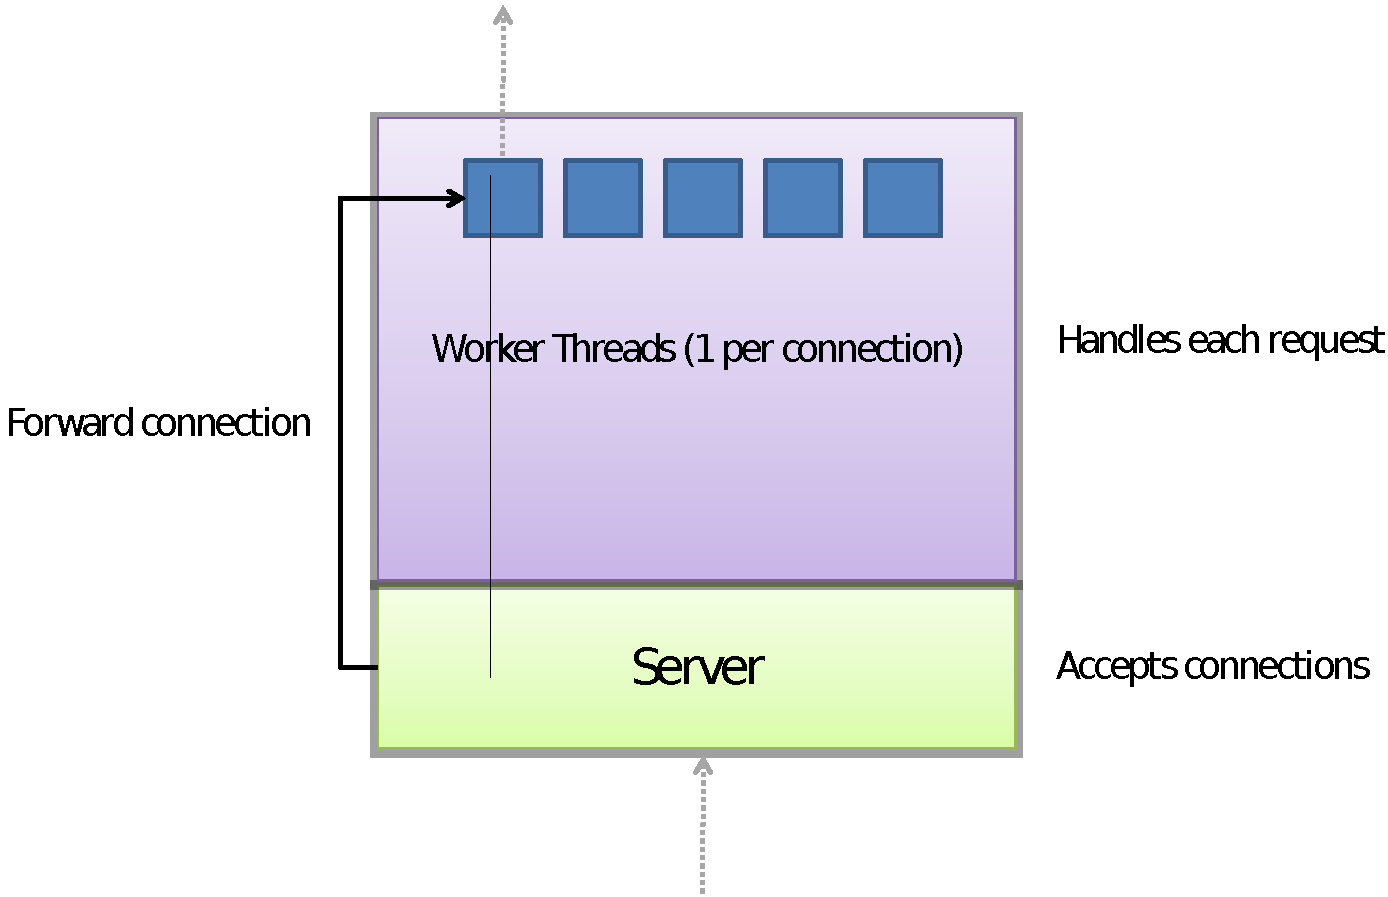
\includegraphics[width=0.75\textwidth]{webrick_architecture}
  \caption{WEBrick's request handling process}
  \label{fig:webrick_architecture}
\end{figure}
Due to its poor performance, users normally used alternate setups which were also known for their lacking stability~\cite{ruby_webservers}.


\subsection{Mongrel}
Mongrel was released by Zed A. Shaw in 2006 and soon became the most popular web server in Rails production environments. It offered much better performance when compared to WEBrick and it was reasonably suited for production environments. This was mainly due to its improved implementation of the HTTP parser, which was now written in C~\cite{mongrel_server_production}.

Similarly to WEBrick, Mongrel uses a single process. It has an acceptor thread which handles every incoming connection, launching new threads for each one of them. In production environments, Mongrel is commonly found in clustered configurations where several processes are launched and their usage is dictated by a proxy server~\cite{mongrel_faq}. Mongrel's request handling is demonstrated on figure~\ref{fig:mongrel_architecture}.
\begin{figure}[h]
  \centering
    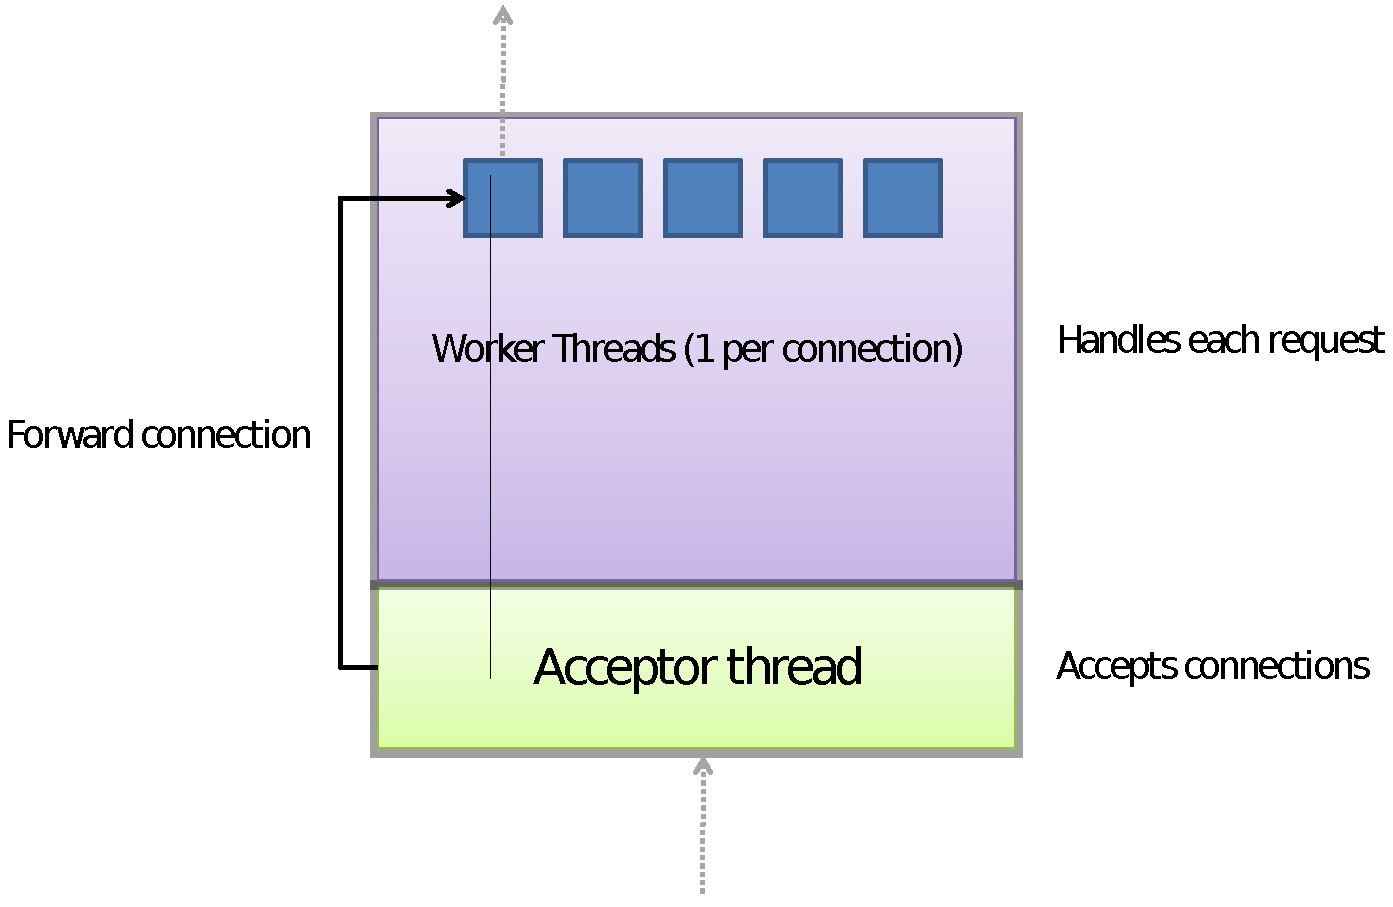
\includegraphics[width=0.75\textwidth]{mongrel_architecture}
  \caption{Mongrel's request handling process}
  \label{fig:mongrel_architecture}
\end{figure}
Mongrel also optimized the TCP stack by changing Ruby's default socket listening queue from 5 to 1024, besides using optimization flags on socket connections to improve bandwidth usage~\cite{mongrel_faq}.


\subsection{Thin}
Thin was released in 2008 and was the first Ruby web server which did not follow the \textit{one thread per request} convention. It uses Mongrel's HTTP parser and EventMachine as its I/O back-end, allowing it to use a fast asynchronous event loop in a single thread for all incoming requests~\cite{thin}. Thin recently became able to combine threading with its philosophy, by allowing the creation of a background pool of 20 threads~\cite{ruby_webservers}. Thin's request handling is demonstrated on figure~\ref{fig:thin_architecture}.
\begin{figure}[h]
  \centering
    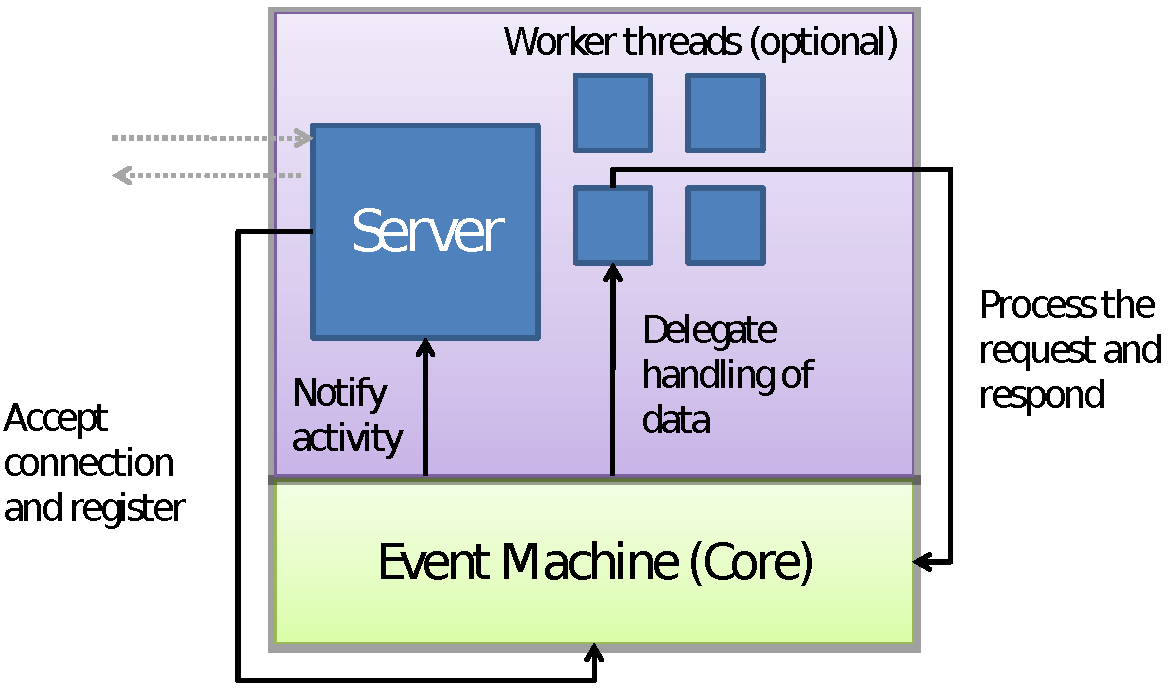
\includegraphics[width=0.75\textwidth]{thin_architecture}
  \caption{Thin's request handling process}
  \label{fig:thin_architecture}
\end{figure}
 This setup yields better performance and scalability than Mongrel, especially when serving small requests like, for example, API calls. This is mainly related to the fact that this web server does not launch a new thread for each request requiring less memory and no context switches~\cite{ruby_webservers}.


\subsection{Passenger}
Passenger was also released in 2008 but it had a big difference from the other options --- it was not a self-contained web server. Passenger relies on other web servers like Apache or Nginx by using their reliable web stack. It is used as a module or extension to these generic web servers, adding the needed functionality to support Ruby and handling certain types of requests~\cite{passenger_whatis}.

When the web server starts, having Passenger loaded as a module, it launches a Ruby process that will be responsible for all the other processes handling the Ruby application, called the \textit{worker processes}. Each request is delivered to the firstly created Ruby processes, which forwards it to one of its worker threads. These worker processes are single threaded and handle one request at a time~\cite{ruby_webservers}. Passenger's request handling is demonstrated on figure~\ref{fig:passenger_architecture}.
\begin{figure}[h]
  \centering
    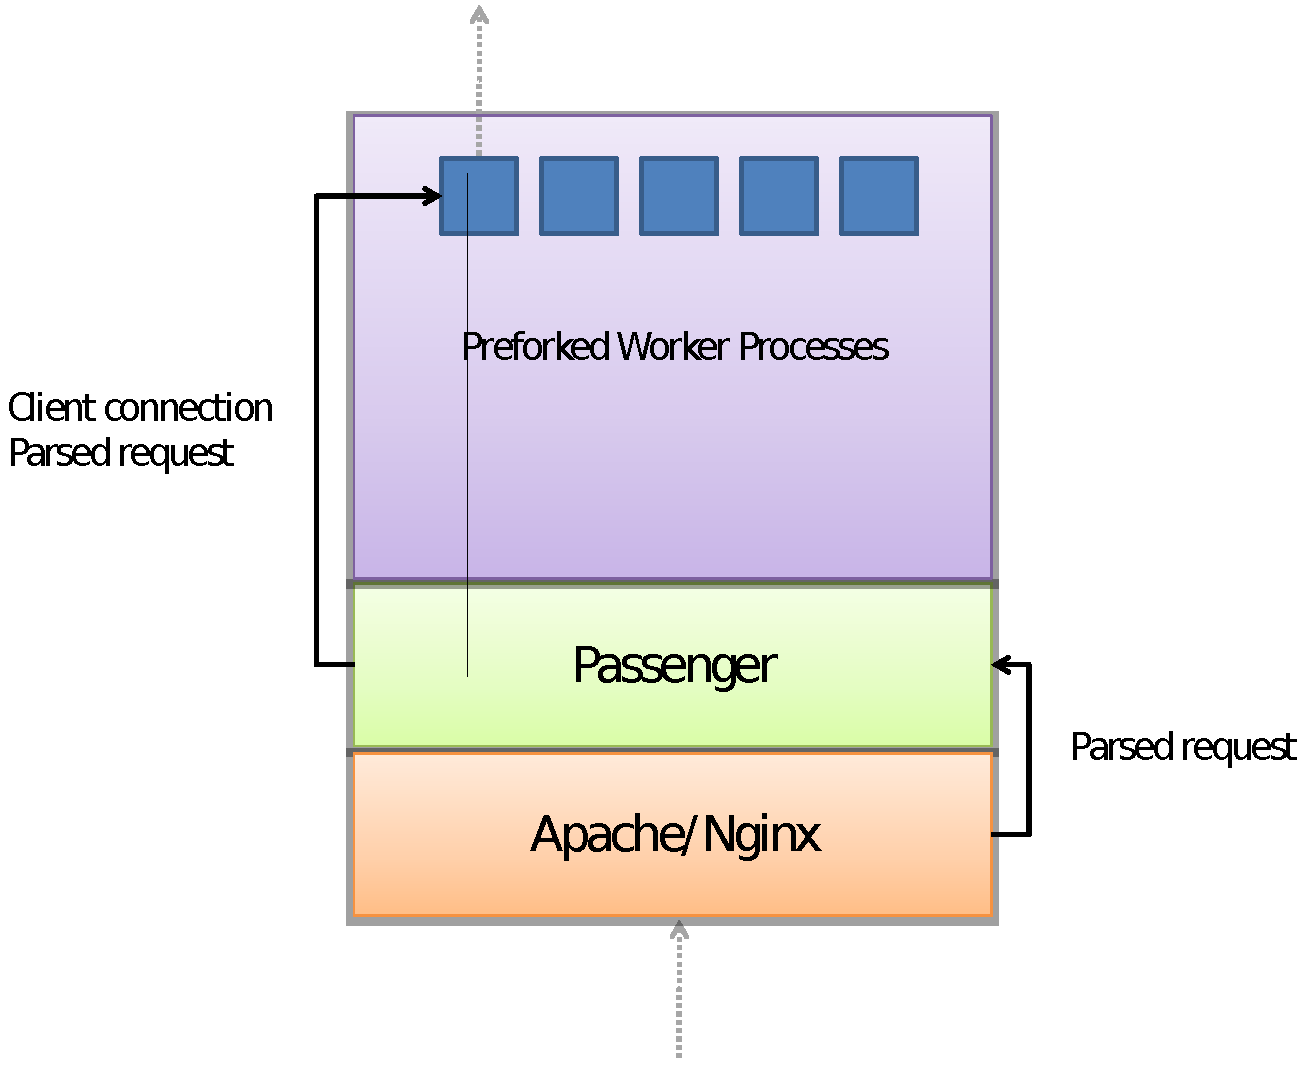
\includegraphics[width=0.75\textwidth]{passenger_architecture}
  \caption{Passenger's request handling process}
  \label{fig:passenger_architecture}
\end{figure}
Passenger is the first real multi-process server for Ruby, although setups with multiple Mongrel or Thin servers were already being used~\cite{passenger_whatis}. Passenger is free but Phusion also provides commercial support.


\subsubsection{Apache}
The Apache HTTP Server is a full-featured and open source web server created by the Apache Software Foundation. It consists on a general purpose web server and provides many useful features such as HTTPS, IPV6 and authentication. Apache natively handles many web development languages such as PHP and Perl~\cite{apache_features}. It can be extended with modules and this is where Passenger comes in --- it will act as \textit{mod\_rails} and extend Apache's functionality to be able to handle Ruby on Rails' applications~\cite{passenger_whatis}.


\subsubsection{Nginx}
Nginx is a lightweight open source web server with a strong focus on performance created by Igor Sysoev~\cite{nginx_features}. Passenger can extend Nginx's functionality by being installed as its module, similarly to the Apache's procedure~\cite{passenger_whatis}.

\section{Databases} % (fold)
\label{tech:sec:databases}
A database is a digitally organized collection of data. It can either be a schema-based or a schema-less database.

\subsection{MySQL}
MySQL is the most popular open source database in the world, having consistently fast performance, high reliability and ease of use~\cite{why_mysql}. It was first released in 1995 and it is the most commonly found database on a Ruby on Rails project. This is the database of choice for all \textit{37signals}'s applications~\cite{interview_dhh}.  It is a relational schema-based database that offers useful features like various storage engines, transactions, indexes, load balancing and many others.

MySQL's architecture consists in three main layers. The top one is related with the services that are not unique to MySQL, like connection handling, authentication and security. The middle layer refers to crucial MySQL features like query parsing, analysis, optimization, caching and all the built-in functions.  This layer also holds all functionality across storage engines and stored procedures. Finally, the bottom layer consists in the storage engines themselves, responsible for the storage and retrieval of all stored data~\cite{high_performance_mysql}. MySQL has four main storage engines---MyISAM, Heap, BDB and InnoDB---with distinct advantages and disadvantages. However, InnoDB is the only storage engine supported in Rails applications. MyISAM and Heap lack transaction support and BDB does not ensure referential integrity, features used by the Ruby on Rails framework. Nevertheless, InnoDB is the default storage engine on MySQL installations.

Ruby has an official library for this database, called \textit{mysql}. There are, however, a few alternatives worth mentioning, namely \textit{mysql2} and \textit{mysqlplus}. These two have some similar and a few other distinct goals:
\begin{description}
  \item[\textit{mysql2}] aims at performing the necessary type conversions between MySQL and Ruby types in C and allows asynchronous queries.
  \item[\textit{mysqlplus}] aims at supporting asynchronous queries and enabling threaded database access.
\end{description}

The installation of \textit{mysql2} automatically patches ActiveRecord, allowing a smooth transition from the default library. The other mentioned alternative, \textit{mysqlplus}, also replaces the default driver and does not need patching to natively interact with ActiveRecord.


\subsection{PostgreSQL}
PostgreSQL is the most advanced open source database server. It was started by Michael Stonebraker at the University of California in Berkeley and had its first release in 1989. It is a DBMS that contains all features found on other open source or commercial databases and a few more~\cite{beginning_postgresql}.

PostgreSQL has some prominent users, like \textit{MySpace}, who strengthen its credibility as a full-featured scalable highly-reliable relational database~\cite{petabyte_warehouses}. Rails' ActiveRecord natively supports this type of database, using Ruby's official library---\textit{ruby-pg}.


\subsection{MongoDB}
MongoDB is a scalable, highly performant, open source, schema-free, document-oriented database written in C++ whose first release was in early 2009. It is a combination of key-value stores, fast, highly scalable and traditional RDBMS systems which provide structured schemas and powerful queries.

This database is document-oriented, providing the simplicity and power of JSON-like data schemas. It supports dynamic queries and indexes. It also provides complex features like replication, auto-sharding and MapRedux~\cite{mongodb}

This database has been gaining popularity within the Rails community for its simplicity of use, high performance and many features that fit well within the Ruby development philosophy~\cite{mongodb_rails}. Mongo is very performance-oriented and some of its features that provide outstanding performance are~\cite{mongodb_couchdb}:
\begin{itemize}
  \item Client driver per language: native socket protocol for client/server interface;
  \item Use of memory mapped files for data storage;
  \item Collection-oriented storage (objects from the same collection are stored contiguously);
  \item Update-in-place;
  \item Written in C++.
\end{itemize}
Rails does not natively support MongoDB. For its usage in Rails the developer must replace its default ORM, \textit{ActiveRecord}, with \textit{MongoMapper}. This library provides access to Mongo database operations and natively supports Ruby objects without conversions~\cite{mongomapper}.



\section{Ruby on Rails} % (fold)
\label{tech:sec:ruby_on_rails}
David Hansson began working on a web-based project management tool oriented towards small teams in 2003. At \textit{37signals} he initially started by using PHP but soon became frustrated by many of the language's shortcomings. He gave up on this language and started implementing what today is known as \textit{Basecamp} in pure Ruby. While developing the application, he noticed that a lot of its code could be extracted into a framework for future use with other applications. Hansson decided to release his framework to the public in July 2004 and Ruby on Rails was born~\cite{railssolutions}.

Rails started to become more mature over time and applications like Twitter, YellowPages, Hulu, Scribd and GitHub were built using this framework. Its popularity has grown significantly since the beginning and its adoption by popular platforms helped establishing Rails as a solid framework.

Ruby on Rails has three main principles which motivated its creation~\cite{agile_webdevelopment_with_rails, ruby_on_rails_principles}:
\begin{description}
\item[Convention over configuration.] In Rails, everything has a default configuration. The only exception is the database connection data. This way, developers only need to specify when they want to use unconventional configurations. This way, Rails offers simplicity while retaining significant flexibility.
\item[Don't Repeat Yourself.] Also known as DRY, this practice implies that the similar code snippets do not exist in separate locations. Every piece of knowledge is unique, definite and has a relevant representation. This simplifies modifications by the avoidance of having to change the same logic in different parts of the project, allowing the applications to keep a high consistency degree.
\item[Model-View-Controller.] Rails follows the MVC architecture pattern, keeping the source code well organized by clearly separating the code according to its purpose. The \textit{Model} is responsible for maintain the state of the application, specifying the constraints its related data has to obey to. The \textit{Controller} receives the users' input, interacts with the model and finally renders a view page as the result. The \textit{View} can have multiple formats, from JSON to XML, and is essentially what is displayed to the users. This principle's schema is presented in figure~\ref{fig:mvc}.
\begin{figure}[h]
  \centering
    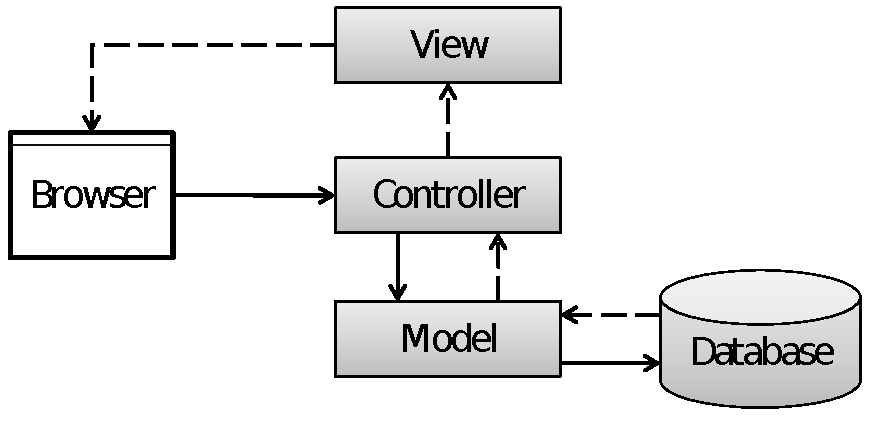
\includegraphics[width=0.75\textwidth]{mvc}
  \caption{Model-View-Controller architectural pattern}
  \label{fig:mvc}
\end{figure}\\
\end{description}
Rails' functionality can be altered and extended with plugins. While being a full stack web framework, Rails does not aim to include every single feature. However, it has been built with a highly extensible infrastructure and it has a considerably large set of plugins nowadays~\cite{rails_magazine_1}.


\subsection{Rails 2}
\label{tech:sec:ruby_on_rails:rails2}
Rails 2 was first released in 2007 and is currently in version 2.3, released at the beginning of 2009. Throughout these 2 years the framework was improved by many contributors, aside from the core team~\cite{rails_core_team}. The framework is essentially divided in six essential modules~\cite{ruby_on_rails_principles, rails23_release_notes}:
\begin{description}
\item[ActionPack] splits the response in two:  a request for the controller to handle the login and a template rendering part for the view to handle.
\item[ActiveRecord] is responsible for object handling and their database representation. Objects are directly linked to the database, so modifying them will modify the table definition they are associated with.
\item[ActiveResource] corresponds to objects that represent the application's RESTful resources as manipulatable Ruby objects.
\item[ActiveSupport] is a collection of various utility classes and standard library extensions.
\item[ActionMailer] is a framework for designing email-service layers, allowing the application to send emails using a mailer model and views.
\end{description}
Rails has a lot of modules and classes but everything is structured using the aforementioned components.


\subsection{Rails 3}
\label{tech:sec:ruby_on_rails:rails3}
Rails 3 is currently in development and it is on its first release candidate, after four beta versions. Most of Rails' code has been refactored and this release's main goals were concerned with improved component decoupling and performance~\cite{rails3_great_decoupling}. 

As of component decoupling, a great deal of work has been done and impressive goals have been achieved~\cite{vaporware_to_awesome}. Most of Rails' components are agnostic now, having standard interfaces for communication with each other. The key concept is that a component is agnostic to whom it is interacting with. This allows component swapping, enabling the replacement of one or more of Rails' core components with a different, third-party one. In order to make this happen standard procedures have been developed, providing standard interfaces for each one of Rails' components.

The decoupling process also allowed for improved modularity, permitting Rails' component separation. ActionController, for instance, has been split into ActionDispatch, ActionController and AbstractController~\cite{vaporware_to_awesome}. There was a lot of work on explicitly handling each component's internal dependencies. This enables the developer to carefully select which modules he needs in his Rails application without caring about including the modules it depends on as well. In previous versions of Rails developers would import the top-level modules, since the alternative was to parse the source code of the framework to find its internal dependencies in order to import all necessary modules. Applications are now able to only load the modules they really need thus becoming faster and lighter.

This improved modularity also had its impact on performance. However, the team also made a specific effort into improving common Rails bottlenecks like partial and collection rendering~\cite{vaporware_to_awesome}, among some other optimized sections.


% chapter technologies (end)

  %% State Of The Art
  \chapter{State of the Art} % (fold)
\label{cha:state_of_the_art}
\headermark{State of the Art}

\section*{} % (fold)
Each component's state of the art will be presented in this chapter, providing an analysis of related work.
% section  (end)

\section{Operating Systems} % (fold)
\label{state:sec:operating_systems}

This research is focused on server environments since deployed Ruby on Rails applications are commonly found in these setups. When it comes to servers, thought, the emphasis on performance becomes much more critical since it is a very important requirement that applications demand from this kind of environment. Some facts suggest that the most commonly found performance bottlenecks in servers are related to the operating system. Operating systems performance bottlenecks usually reside in three key issues~\cite{os_performance_server}:
\begin{itemize}
\item Process management;
\item Virtual memory management;
\item High performance I/O.
\end{itemize}
Each operating system addresses bottlenecks differently and their decisions impact application specific and system-wide performance.

In this research's context, performance is addressed from a Ruby on Rails perspective. Windows' support for this framework and related components is poor and this environment makes the framework slower. Passenger, one of the major Rails web servers used in production, opted not to support the Windows platform. As Marcus Koze explains~\cite{marcus_koze_passenger}:
\begin{quote}
  ``We have no plans to port Passenger on Windows. Windows lacks the proper facilities to implement Passenger efficiently. Passenger on Windows will be very, very inefficient, which can give both Ruby on Rails as well as Passenger a bad name.''
\end{quote}
Many other web-oriented benchmarks show that Linux has better scalability and performance compared to Windows when it comes to this type of servers~\cite{apache_tomcat_performance_linux_windows, php_apache_linux_windows}. The difference is quite noticeable: Ruby on Rails is still more efficient in a Virtual Machine running Linux than in a normal installation of Windows~\cite{linux_virtualbox_windows_rails}.

Documentation on how to use and deploy Rails applications in the Windows platform is also scarce, often needing unconventional methods for being able to run it properly~\cite{rails_windows}.

Since Rails is built on top of the Ruby programming language, this framework's lack of performance in Windows is possibly related to the poor Ruby performance in this operating system. The Ruby 1.8 official interpreter is twice as fast in Linux than its Windows counterpart. As of YARV, the Ruby 1.9 official interpreter seems to be 70\% faster on Linux when compared to its Windows counterpart~\cite{ruby_faster_linux}. Windows-specific Ruby interpreters do not seem to have noticeable performance improvements~\cite{ruby.net} and lack the necessary stability and compliance with the Ruby specification. \textit{IronRuby}, for instance, is an interpreter developed by Microsoft~\cite{ror_ecosystem_whitepaper} that is faster than Windows' MRI but still slower than the YARV implementation for this operating system. It also presents stability issues, as timeouts are common in a considerable number of benchmarks~\cite{ironruby_performance}.

On a side note, MySQL's documentation states that there are a few unpleasent details when using this database under a Windows environment~\cite{mysql_windows_linux}. First of all, it is only conceded 4000 ports which after being used need two to four minutes before becoming available again. It also has a limited allowed opened files number---2048---restraining its concurrent capabilities. Finally, MySQL uses a blocking read for each connection and Windows' connection error handling is quite poor when compared to Linux's counterpart. As the aforementioned documentation states, all these differences limit the number of acceptable concurrent requests handled and difficult high-load handling. They can lead to performance issues and limit the system's scalability.

To date, there are no specific tests analyzing Ruby on Rails' performance on BSD when compared to other operating systems. However, many web discussions suggest that it is quite similar to the one achieved on Linux which is understandable since they are both \textit{UNIX} derivates.

\section{Ruby} % (fold)
\label{state:sec:ruby}
The Ruby on Rails framework, as its name implies, is built on top of the Ruby programming language. Rails' performance is highly affected by Ruby and the interpreter choice can lead to great impact on the framework's scalability.

Ruby has many interpreters according to its version. Ruby 1.8 has MRI as its default interpreter and Ruby 1.9 has YARV. There are, however, a few other implementations that start to deserve some attention. These present different philosophies and implementation details that provide them with a few advantages and other shortcomings. The most popular Ruby interpreters for Ruby 1.8 are as follows:
\begin{description}
\item[MRI,] the standard Ruby 1.8 interpreter.
\item[Ruby Enterprise Edition,] based on the MRI's code but modified for better performance in Rails environments.
\item[JRuby,] a Ruby interpreter built on top of JVM.
\item[Rubinius,] a promising Ruby interpreter built by Rails' creators --- \textit{EngineYard}.
\end{description}
Version 1.9 came out recently so alternative interpreters do not fully support it just yet. YARV, the standard Ruby 1.9 interpreter, is the only one to support the specification.

The default implementation for Ruby 1.8, MRI, is generally known by its poor performance~\cite{6tips_for_mri}. This motivated the development of efficient interpreters for the language. Ruby Enterprise Edition has better scaling abilities than MRI, generally performs better and uses less memory~\cite{ree_benchmarks}. JRuby outperforms MRI by a considerable margin~\cite{ruby19_performance}. Rubinius, on the other hand, also effortlessly outperforms MRI. It also performs better than JRuby in most cases but by a much smaller margin~\cite{rvm_rubinius_benchmarks}.

Some people found significant performance improvements in MRI by applying a series of patches and configurations to its garbage collector. Twitter benefited from this patches, roughly improving its overall performance by 30\%~\cite{ruby_gc_tuning}.

Ruby 1.9 has only one compliant interpreter as aforementioned. However, as reference benchmarking, its performance is better than JRuby's~\cite{ruby19_performance}  and is paired with Rubinius'. It performs slightly better in some benchmarks but also performs faintly worse on others~\cite{rvm_rubinius_benchmarks,ruby_interpreter_benchmarks}. Some people even got as far as saying it was more efficient than Python's counterpart~\cite{ruby19_python}.


\section{Rails Web Servers} % (fold)
\label{state:sec:rails_web_servers}
The first Rails web server was WEBrick, publicly released in 2000. Mongrel came in 2006 and soon after Thin and Passenger followed.

Using the aforementioned web servers, Muhammed Ali did an extensive overview of some characteristics that heavily contribute to web server performance~\cite{ruby_webservers}. Muhammed's analysis is exposed in the following sections, along with a brief overview of how each web server handles them.

\subsection{Data Copying}
When a server fetches a file from the disk or a back end server it usually copies it to kernel space in order to send it to the client. There are ways of sending the data directly without copying it, called \textit{zero-copy} techniques~\cite{ zero-copy_data_transfer}.

WEBrick, Mongrel and Thin neglect this issue. Passenger neglects it as well but, on the other hand, it passes file descriptors to worker processes which avoids sending the data to the clients through the parent web server.

\subsection{Context Switching}
This issue is related with context switching between kernel and user space and all the overhead involved in this procedure. System calls and thread exchange are some of the activities that cause context switches.

WEBrick and Mongrel highly rely on threads, which implies many context switches. In Passenger's case, context switches are related to process context switching, since it uses processes instead of threads. Thin efficiently handles context switches---it does not use threads nor processes, reducing the impact of this issue.

\subsection{Lock Contention} 
Multiple threads or processes with shared data imply data locking from time to time. If the data is locked it will put the remaining threads or processes trying to use it on hold.

WEBrick's and Mongrel's threads share almost no data, avoiding noticeable issues related to lock contention. Neither Thin nor Passenger share data inter processes or threads, completely avoiding lock contention.

\subsection{Memory Management}
Web servers allocate and free memory frequently and Ruby's garbage collector is not very efficient for such application behavior. Web servers might counter this issue by allocating little objects and/or reusing them as much as possible.

WEBrick does not conserve memory neither reuses objects. In Mongrel, though, parser objects are reusable and string usage is kept to a minimum, being replaced by constants. Thin also avoids using strings in detriment of constants but buffers data twice in memory before retrieving it from \textit{Rack}. Passenger does an excellent job in memory management by using the fork friendly Ruby implementation, allowing it to recycle worker processes.

\subsection{Blocking Operations}
I/O operations, as mentioned before, block the server until the operation finishes.

WEBrick solely relies on non-blocking I/O. Contrary, Mongrel performs all I/O in a blocking manner because of its usage of threads. Thin, on the other hand, does most of its I/O operations in a non-blocking manner and Passenger is not affected by this issue since it uses single threaded processes.

\subsection{HTTP Parsing}
The implementation of the HTTP parser greatly affects the web server performance since it is a heavy procedure.

WEBrick's HTTP parser is written in pure Ruby, having poor performance. Mongrel, in contrast, uses a fast and secure implementation written in C. While Thin uses a similar parser to Mongrel's one, Passenger does not do HTTP parsing and handles that responsibility to its underlying web server.

\subsection{TCP Stack}
Web servers can tune TCP operations by specifying a set of options allowed by the TCP protocol implementation.

WEBrick and Thin do not try to optimize the TCP stack while Mongrel uses two configuration options that increase the number of allowed waiting connections and \textit{TCP\_CORK} to optimize bandwith usage. Finally, these kinds of optimizations on Passenger depend on whether its underlying web server is using TCP stack optimization configurations.\\\\% FIXME: hack :|
From all the exposed Rails web servers, Passenger presents itself as the easiest to setup in a server environment~\cite{ruby_webservers} since it can be installed as a module for other easily installable web servers like Apache or Nginx.

\subsection{Benchmarks}
Some benchmarks were endured by Muhammed Ali~\cite{ruby_webservers}, whose results are showed on table~\ref{tab:webserver_benchmarks}.
\begin{table}[h!t]
  \centering
  
  \begin{tabular}{p{1.3cm}|p{1.8cm}|p{2cm}|p{2cm}|p{2cm}|p{1.3cm}|p{2cm}}
    \textsc{Test}
  & \textsc{Users}
  & \textsc{Requests}
  & \textsc{WEBrick}
  & \textsc{Mongrel}
  & \textsc{Thin}
  & \textsc{Passenger} \\
  \hline

  \multirow{3}{*}{1}
  & 10 & 1000 & 169 & 438 & 650 & 497\\
  & 100 & 1000 & 209 & 451 & 613 & 509\\
  & 1000 & 1000 & 250 & 446 & 615 & 324\\
  \hline
    
  \multirow{3}{*}{2}
  & 10 & 1000 & 115 & 309 & 365 & 305\\
  & 100 & 1000 & 165 & 299 & 350 & 316\\
  & 1000 & 1000 & 194 & 284 & 346 & 307\\
  \hline
  
  \multirow{2}{*}{3}
  & 10 & 1000 & 41 & 44 & 43 & 45\\
  & 100 & 1000 & 41 & 42 & 45 & 44\\
  \hline

  \multirow{2}{*}{4}
  & 10 & 1000 & 41 & 37 & 55 & 79\\
  & 100 & 1000 & 41 & 37 & 54 & 79\\
  \hline
  
  \multirow{2}{*}{5}
  & 10 & 1000 & 6 & 5 & 7 & 10\\
  & 100 & 1000 & 6 & 5 & 2 & 10\\
  
  \end{tabular}
  \caption{Web server benchmark results}
  \label{tab:webserver_benchmarks}
\end{table}
All tests consist in serving dynamic requests from a single Rails process. All requests are made concurrently and each web server's results are in number of requests handled per second. Test 1 is a sample ``Hello World!'' page. Test 2 fetches a database record and renders it as an ERB template. Test 3 marshals 500 complex objects. Test 4 sends a large 1MB response. Finally, test 5 sends a very large 10MB response.

According to Muhammed's analysis, WEBrick is evidently slow when compared to its counterparts. Mongrel performs much better that its ancestor and both Thin and Passenger improve over it. Thin is clearly the best web server for serving small requests. Passenger, though, is the one to scale better since it performs similarly with 10 or 1000 concurrent users. It also shows better performance when handling large responses. Its performance could be different if it was using Nginx as its back-end instead of Apache.

Unicorn was not contemplated on the previously shown tests but it has been gaining reputation and its adoption is increasing. \textit{Twitter}, the problematic platform mentioned before, recently switched over to Unicorn as its web server, publicly praising some of its features. Among them are its request queue handling, master/slaves architecture, error encapsulation and recovery, CPU usage and a feature called \textit{zero-downtime deployment} that ``works beautifully''~\cite{twitter_unicorn}.


\section{Databases} % (fold)
\label{tech:sec:databases}
A database collects data, either records or files. From the Rails perspective, this can either be a schema-based or a schema-less database.


\subsection{MySQL}
MySQL is the most popular open source database in the world, having consistently fast performance, high reliability and ease of use~\cite{why_mysql}. It was first released in 1995 and it is the default database on a Ruby on Rails project. This is the database of choice for all \textit{37signals}'s applications~\cite{interview_dhh}.  It is a relational schema-based database that offers useful features like various storage engines, transactions, indexes, load balancing and so on.

Figure~\ref{fig:mysql_architecture} presents a simple overview over MySQL's architecture.
\begin{figure}[h]
  \centering
    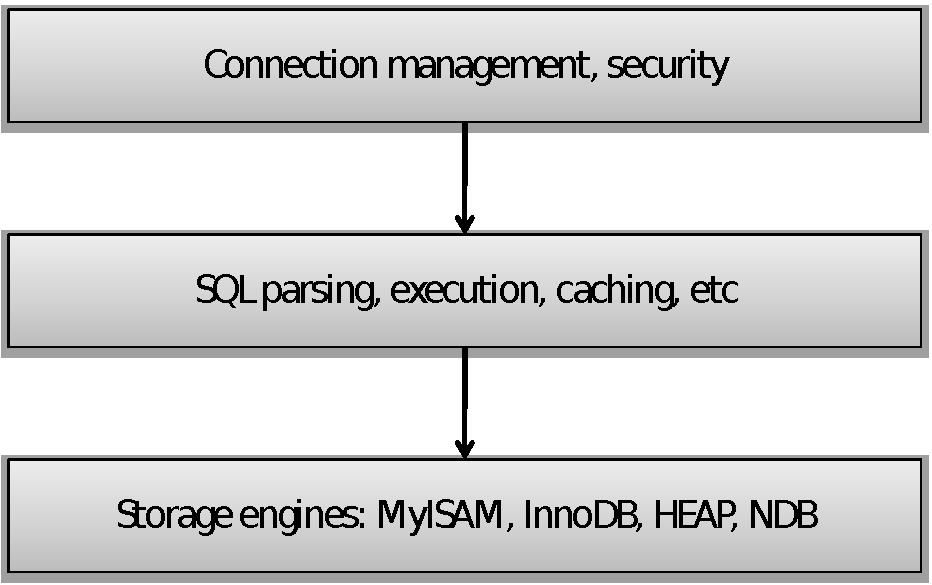
\includegraphics[width=0.75\textwidth]{mysql_architecture}
  \caption{Logical view of MySQL's architecture}
  \label{fig:mysql_architecture}
\end{figure}
The top layer is related with the services that are not unique to MySQL, like connection handling, authentication and security. The middle layer refers to crucial MySQL features like query parsing, analysis, optimization, caching and all the built-in functions.  This layer also holds all functionality across storage engines and stored procedures. Finally, the bottom layer consists in the storage engines themselves, responsible for the storage and retrieval of all stored data~\cite{high_performance_mysql}. MySQL has four main storage engines, all with advantages and disadvantages, the default one being InnoDB.

A high-level summary of the characteristics of all four storage engines can be found on table~\ref{tab:storage_engines_mysql}.
\begin{table}[ht]
  \centering
  
  \begin{tabular}{p{4cm}|p{2cm}|p{2cm}|p{3cm}|p{2cm}}
    \textsc{Attribute}
  & \textsc{MyISAM}
  & \textsc{Heap}
  & \textsc{BDB}
  & \textsc{InnoDB} \\
  \hline

    \textbf{Transactions}
  & No
  & No
  & Yes
  & Yes \\

  \hline
    \textbf{Lock granularity}
  & Table
  & Table
  & Page
  & Row \\

  \hline
    \textbf{Storage}
  & Split files
  & In-memory
  & Single file per table
  & Tablespace \\

  \hline
    \textbf{Isolation levels}
  & None
  & None
  & Read committed
  & All \\

  \hline
    \textbf{Portable format}
  & Yes
  & No
  & No
  & Yes \\

  \hline
    \textbf{Referential integrity}
  & No
  & No
  & No
  & Yes \\

  \hline
    \textbf{Primary key with data}
  & No
  & No
  & Yes
  & Yes \\
    
  \hline
    \textbf{MySQL caching}
  & No
  & Yes
  & Yes
  & Yes \\

  \hline
    \textbf{Available versions}
  & All versions
  & All versions
  & MySQL-Max
  & All versions \\
  \end{tabular}
  \caption{Storage engine characteristics in MySQL}
  \label{tab:storage_engines_mysql}
\end{table}
Rails' ActiveRecord natively supports this type of database.


\subsection{PostgreSQL}
PostgreSQL is the most advanced open source database server. It was started by Michael Stonebraker at the University of California in Berkeley and had its first release in 1989. It is a DBMS that contains all the features found on other open source or commercial databases and a few more. Some of these features include~\cite{beginning_postgresql}:
\begin{itemize}
  \item Transactions;
  \item Subselects;
  \item Views;
  \item Foreign key referential integrity;
  \item Sophisticated locking;
  \item User-defined types;
  \item Inheritance;
  \item Rules;
  \item Multiple-version concurrency control;
  \item Native Microsoft Windows version;
  \item Table spaces;
  \item Ability to alter column types;
  \item  Point-in-time recovery.
\end{itemize}
PostgreSQL has some prominent users, like MySpace, who strengthen its credibility as a full-featured scalable highly-reliable relational database~\cite{petabyte_warehouses}. Rails' ActiveRecord natively supports this type of database.


\subsection{MongoDB}
MongoDB is a scalable, high performance, open source, schema-free, document-oriented database written in C++ whose first release was in early 2009. It is a combination of key-value stores, fast and highly scalable, and traditional RDBMS systems which provide structured schemas and powerful queries. Among other features, MongoDB provides~\cite{mongodb}:
\begin{itemize}
  \item Document-oriented storage (the simplicity and power of JSON-like data schemas);
  \item Dynamic queries;
  \item Full index support, extending to inner-objects and embedded arrays;
  \item Query profiling;
  \item Fast, in-place updates;
  \item Efficient storage of binary data large objects (e.g. photos and videos);
  \item Replication and fail-over support;
  \item Auto-sharding for cloud-level scalability;
  \item MapReduce for complex aggregation.
\end{itemize}
This database has been gaining popularity within the Rails community for its simplicity of use, high performance and many features that fit well within the Ruby development  philosophy~\cite{mongodb_rails}. Mongo is very performance oriented and some of its features that provide outstanding performance are~\cite{mongodb_couchdb}:
\begin{itemize}
  \item Client driver per language: native socket protocol for client/server interface (not REST);
  \item Use of memory mapped files for data storage;
  \item Collection-oriented storage (objects from the same collection are stored contiguously);
  \item Update-in-place (not MVCC);
  \item Written in C++.
\end{itemize}
Rails' ActiveRecord does not natively support MongoDB. For its usage in Rails the developer must use \textit{MongoMapper}, which provides access to Mongo database operations and natively supports Ruby objects without conversions~\cite{mongomapper}.


\section{Ruby on Rails} % (fold)
\label{state:sec:ruby_on_rails}
Rails' development is mainly done by its creators --- \textit{37signals} --- and so are its performance optimizations. However, many companies like Twitter had the need to squeeze this frameworks scalability and focused on some identified critical bottlenecks like Ruby's garbage collector mentioned in section~\ref{state:sec:ruby}.

There have been some outside performance improvements over Rails 2.3 code, though. From simple Rails' source minor patching~\cite{accunote_rails} to complete architecture makeovers ~\cite{distributed_rails}, Ruby on Rails' improvement attempts were widely made.

However, the main performance improvements over Rails 2.3 can be found in Rails 3. The decoupling mentioned in section~\ref{tech:sec:ruby_on_rails:rails3} improved Rails performance and scalability, allowing faster execution times and lighter memory usage.

There were also specific performance optimizations, namely on \textit{partial} and \textit{collection} handling. Controller code was also refactored to become lighter. Initial performance benchmarks show that partial and collection rendering and overall performance is more than two times faster~\cite{rails_merb_merge_performance, vaporware_to_awesome}.


% chapter state_of_the_art (end)

  %% Proposed Approach
  \chapter{Approach} % (fold)
\label{cha:approach}
\headermark{approach}

\section*{} % (fold)
The proposed approach consists in envisioning scaling and performance optimization as a whole, where all components take part in scaling and improving the system. Having that said, it is necessary to look out for sensitive dependencies, or the aforementioned \textit{butterfly effect} when optimizing the system.

As an example, the Ruby MRI interpreter's garbage collector consists in an implementation of the \textit{mark-and-sweep} algorithm which is good enough for most applications but lacks the efficiency to deal with heavy and memory intensive applications like Rails~\cite{passenger_whatis}. It is a perfectly reliable garbage collector for the majority of Ruby applications, but it is not the best choice for Rails itself.

Every component must be seen from the Rails perspective and bottlenecks must be identified and contoured.

To achieve this, we need to set up an initial setup for benchmarking, tweaking and patching. This involves using a specific operating system and that choice will be made based on three essential factors:
\begin{enumerate}
  \item The information gathered in the state of the art of Operating Systems, from the Rails perspective;
  \item A small set of benchmarks for standard performance analysis;
  \item Configuration easiness, as some operating systems and distributions tend to stimulate system tweaking by allowing easy access to certain features and configurations and others, on the other hand, might not have this feature in their goals and consequently make it harder to tweak and configure at will.
\end{enumerate}
After starting with the chosen operating system, kernel settings will fill the first chapter of the abovementioned guidelines as they have a great impact on operating system behavior. Important settings regarding TCP/IP behavior, I/O scheduler, Preemption, Interrupt Timers \textit{et al.} must be tested and benchmarked from the Rails perspective in order to achieve a configuration set that suits Rails --- and all the other components --- best.

When the mentioned set of configurations and settings is met, the web servers will become the research and development target. Not all of them will be tested since the state of the art on web servers rules some of them out, but at least two will be taken into a small set of benchmarks and configuration tweaking. After finding which suits Rails best, research will deepen and eventual bottlenecks might be found and improving patches will be developed.

Following the web server choice, ruby interpreters will become the aim. Once again, the state of the art on ruby interpreters rules some of them out but at least two will endure a small set of benchmarks and configuration tweaking to conclude which scales better and has a better performance from the Rails point of view. Possible bottlenecks will be found and, once again, an attempt at solving the most critical ones will be made. After that, a series of patches will be released in order to improve that interpreter even further.

The next target is a commonly know bottleneck on web applications – the database. A few will be tested, following the \textit{at least two} rule, but here there is a clear division on two essential types of databases:
\begin{enumerate}
  \item Schema-based databases, like the famous MySQL or PostgreSQL;
  \item Schema-free document-oriented databases, like MongoDB or CouchDB.
\end{enumerate}
While schema-based databases are very popular and reliable, not to mention that they are tested thoroughly because of being so popular and so mature, schema-free databases emerge as high performance solutions with little pitfalls. Both types must be tested and benchmarked, in order to provide results and configurations that suit most Rails applications, whether they are using a schema-based database or not. Bottlenecks will also be searched and attempts at fixing them will be made. An approach to caching will also be made in the database regard, as it is a crucial concept when scaling. If major bottlenecks are found in the existing caching solutions, an improvement attempt will be made and possible positive outcomes will be submitted as patches to the developing community.

The next phase is related to Rails itself. Since, as mentioned, Rails 3.0 is a big improvement over Rails 2.3 from a performance perspective, no attempts at improving Rails 2.3 will be made. However, remaining bottlenecks in Rails 3.0 will be targeted for improvement with guidance from the Rails core development team.
Finally, the case-study application, Escolinhas~\cite{escolinhas}, will be aimed for improvement. The architecture and code will be reviewed to find and erase performance bottlenecks, always taking Rails' strengths and weaknesses into account to fully optimize the application for the framework it is being developed on. This will allow the development of a small set of generalist guidelines and programming conventions that suit most Rails developers and their respective applications.
Different components become the main focus at different times. A brief summary of the above information is presented in table~\ref{tab:research_development_schedule} which indicates when a given component will become the main focus and for how long that is expected to happen.
\begin{table}[h]
  \centering
  \begin{tabular}{p{8cm}|p{2.1cm}p{3.5cm}}
    \textsc{Target component}
  & \textsc{Start date}
  & \textsc{Duration (weeks)}
  \\
  \hline
    \textbf{OS Choosing}
  & 15/02/2010
  & 1
  \\
  \hline
    \textbf{OS kernel testing and tunning}
  & 22/02/2010
  & 1
  \\
  \hline
    \textbf{Web server testing and bottleneck research}
  & 01/03/2010
  & 1
  \\
  \hline
    \textbf{Web server bottleneck improvements}
  & 08/03/2010
  & 1
  \\
  \hline
    \textbf{Ruby interpreter testing and bottleneck research}
  & 15/03/2010
  & 1
  \\
  \hline
    \textbf{Ruby interpreter bottleneck improvements}
  & 22/03/2010
  & 1.5
  \\
  \hline
    \textbf{DB testing and bottleneck research}
  & 31/03/2010
  & 1
  \\
  \hline
    \textbf{DB bottleneck improvements}
  & 07/04/2010
  & 1
  \\
  \hline
    \textbf{Rails 3.0 bottleneck research}
  & 14/04/2010
  & 1
  \\
  \hline
    \textbf{Rails 3.0 bottleneck improvements}
  & 21/04/2010
  & 2.5
  \\
  \hline
    \textbf{Escolinhas analysis and bottleneck research}
  & 10/05/2010
  & 1
  \\
  \hline
    \textbf{Escolinhas platform improvements}
  & 17/05/2010
  & 3
  \\
  \hline
    \textbf{Write dissertation report}
  & 07/06/2010
  & 4
  \\
  \end{tabular}  
  \caption{Component focus scheduling}
  \label{tab:research_development_schedule}  
\end{table}\\
In order to benchmark every component, others which run on top of it must be taken into account. This way, the research starts by involving every single component. After having conclusive results for each one of them they will be removed from the research, as shown on figure~\ref{fig:gantt}. The main focus will then leap into another component.
\begin{figure}[th]
  \begin{center}
    \leavevmode
 
    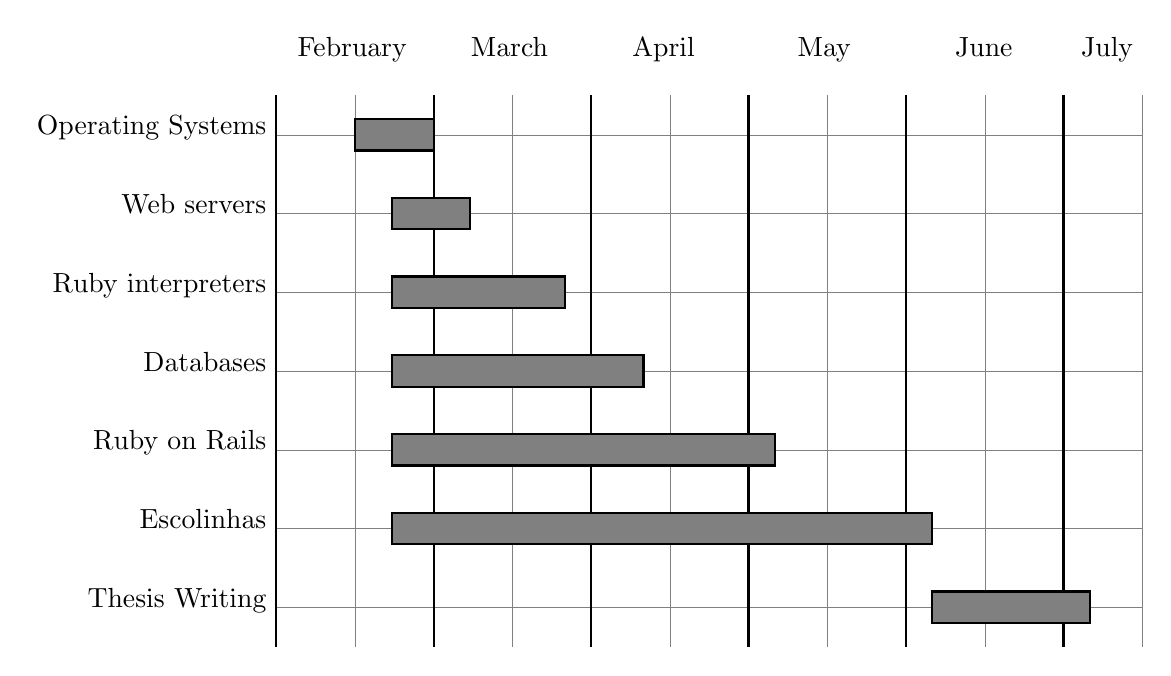
\begin{tikzpicture}[y=-1cm]
      \draw[help lines] (0,7.5) grid (11,0.5);
      \draw[thick] (0,0.5) -- (0,7.5);
      \draw[thick] (2,0.5) -- (2,7.5);
      \draw[thick] (4,0.5) -- (4,7.5);
      \draw[thick] (6,0.5) -- (6,7.5);
      \draw[thick] (8,0.5) -- (8,7.5);
      \draw[thick] (10,0.5) -- (10,7.5);
      
      \node at (0.15,0.0) [anchor=base west] {February};
      \node at (2.35,0.0) [anchor=base west] {March};
      \node at (4.4,0.0) [anchor=base west] {April};
      \node at (6.5,0.0) [anchor=base west] {May};
      \node at (8.5,0.0) [anchor=base west] {June};
      \node at (10.1,0.0) [anchor=base west] {July};
      
      \ganttline{1}{Operating Systems}{15}{30}
      \ganttline{2}{Web servers}{22}{37}
      \ganttline{3}{Ruby interpreters}{22}{55}
      \ganttline{4}{Databases}{22}{70}
      \ganttline{5}{Ruby on Rails}{22}{95}
      \ganttline{6}{Escolinhas}{22}{125}
      \ganttline{7}{Thesis Writing}{125}{155}
    \end{tikzpicture}
 
    \caption{Work scheduling}
    \label{fig:gantt}
  \end{center}
\end{figure}\\
All the mentioned testing, tuning, bottleneck research and improvements are directly related to scaling and performance optimizations, as suggested throughout this thesis.
Once again, it becomes critical to reaffirm that each area will be essentially targeted from the Rails perspective, taking sensitive dependences into account in order to avoid optimizing a specific component while taking the risk of making the system, as a whole, slower or less scalable.


  %% Conclusions
  \chapter{Conclusions} % (fold)
\label{cha:conclusions}
\headermark{Conclusions}
\section*{} % (fold)

\begin{comment}
This is deprecated!!!!!!

The existing research provides a solid base for future work on this subject. The endured technology overview allowed the creation of an expectancy base for each component. The state of the art provided an overview of the current engaged work on related, if not similar, subjects.

All the gathered and structured information permitted option narrowing when it comes to future work. Taking into account the research and conclusions of some related work, some components will be left out of future benchmarking, tuning, testing and improvement.

On the Operating System's concern, Microsoft's operating system will be left out of future efforts since its Ruby and Rails support is significantly poor and inefficient. The lack of benchmark and testing information about BSD and the fact that its performance should be similar to Linux's include it in the test group. Concluding, the Operating Systems contempt by this project will be Linux and BSD.

Ruby is currently in version 1.9 which has many improvements over the previous version, both performance and not performance-oriented. Since YARV is the only one to support its specification to full extent, this will be the only interpreter targeted for improvements. Luckily, Rubinius' 1.9 support is growing day by day and it is close to 100\%. Only time will tell if this interpreter will be considered as well.

Rails web servers' situation is more flat. Only WEBrick is left out for obvious reasons --- it was Rails' pioneer web server but lacks the efficiency to compete with nowadays alternatives.

When it comes to relational databases, MySQL's scaling and performance capabilities shine. On the other hand, MongoDB presents itself as a worthy alternative but it has an important characteristic --- it is a schema-less database. PostgreSQL, although providing many interesting features, is not efficient enough to compete with MySQL, being left out of the test group for further work. MySQL and MongoDB are targeted for all the aforementioned improvement cycle.

Rails is growing fast and version 3 will soon to be publicly released. It solves many existing performance bottlenecks in Rails 2.3 and improves its predecessor code by a great deal. Working on Rails 2.3 would not be very productive since it will soon become deprecated and inefficient when compared with the most recent version. Version 3 will be the main target focus for further development.

The application itself, \textit{Escolinhas}, would benefit from huge performance gains just by being ported to Ruby 1.9 and Rails 3. The remaining improvements are dependant on the improvement cycles of all the components mentioned before, as performance bottlenecks must be found and solved on each setup.

Ultimately this research provided a careful overview over the involved technologies and their current state, sustaining the creation of a solid research and development plan for future efforts.
\end{comment}

\section{Conclusions}
Guidelines and conventions are created

Escolinhas is more scalable

Open-source contribution with considerable range and big impact


\section{Summary of Contributions}

Created generic guidelines and conventions

Improved Rails profiling abilities

Improved Ruby's profiling abilities

Improved Ruby's GC flexibility

Ported Escolinhas to Ruby 1.9

Ported Redmine to Ruby 1.9 and Rails 3

Ported the plugins used by Escolinhas to Rails 3

Demonstrated Ruby's performance on different OSes

Demonstrated OSes performance with generic and web-oriented benchmarks

Creation of web server benchmarking scripts

In-depth analysis of the current web servers performance

Demonstrated the performance of the latest Ruby against the most used version

Joint of many micro-researches (?)


\section{Future Research}

Research other databases aside mysql

Invest in alternative Ruby interpreters (which should be stable in a near future)

Develop a generational GC for Ruby


  
  
  %%----------------------------------------
  %% Final materials
  %%----------------------------------------

  \begin{singlespace}
    \PrintBib{references}

    %% Index
    %% Uncomment next command if index is required,
    %% don't forget to run ``makeindex mieic'' command
    %\PrintIndex

    %% Comment next 2 commands if numbered appendixes not used
    %\appendix
    %\include{appendix_a}
    %\include{appendix_b}
  \end{singlespace}
\end{document}
